\section{Overview}
Solving complex optimization problems has been a hot topic the past decade and has garnered large followings most of which are practitioners and researchers. This attention has brought upon the development of new metaheuristic algorithms, many of which are inspired by various phenomena demonstrated by nature.
The paper proposes a new population based algorithm, the Lion Optimization Algorithm (LOA) \cite{loa_2016}. The distinct lifestyle of lions and their characteristics of utilizing cooperation was made as the motivational basis for the development of this optimization algorithm. The algorithm is also tested against benchmark problems sourced from literature and whose primary solutions was compared with the results of the test. The results also confirm the performance of this algorithm alongside other algorithms used in the paper.

\section{Optimization}
Basically, optimization is searching for the best solutions out of all possible solutions. A best solution can be defined regarding either the most of some measure of success (e.g. revenue) or the least of another measure (e.g. cost). We can be looking at a group of answers or one answer from a set. In solving optimization problems, one's goal is to minimize or maximize a result variable of a function by trying out different parameters for input.

\section{Optimization Algorithms}
Optimization algorithms can be divided into two major categories, as exact and approximate \cite{desale_2015}. Exact algorithms guarantee that the optimal solution to the problem will be found in a finite amount of time. There are, however, harder optimization problems that requires the searching of very large solution sets and thus making it impractical to use exact algorithms. An example of this is the travelling salesman problem, whereby a salesman is tasked to plan a path that visits a series of cities exactly once and return to his starting point with minimum distance travelled. In this problem, the number of possible paths that the salesman can take grows factorially as the number of cities increases. It is possible to solve this problem using brute-force method but it would take a lot of time. As such, the usage of approximate algorithms are necessitated. These algorithms do not guarantee that the optimal solution will be found, but it can find an approximate (sometimes exact) solution to the problem in a relatively short amount of time, sometimes using a less computationally intensive method. Approximate algorithms can be further divided into two major categories as heuristic and metaheuristic algorithms \cite{desale_2015}.

Heuristic algorithms are problem-dependent techniques that approximate the solution to a problem using readily available information. Meaning, they try to take advantage of the particularities of the problem to find a solution. Applications of these algorithms include finding the best move in a chess game, solving a tic-tac-toe puzzle, and pathfinding. In these examples, the underlying concepts of the problem are first analyzed and then used to guide the algorithm in searching for a solution. 

Metaheuristic algorithms, on the other hand, requires minimal or no assumptions about the problem being solved. They can be tailored to optimize a specific problem which makes them applicable to a wide variety of problems. A metaheuristic algorithm optimizes a problem by iteratively improving a candidate solution until a desired quality is achieved. Metaheuristic algorithms often employ mechanisms to escape from being stuck in a local optimum and thus making them more likely to obtain the global optimum solution. 

An example of an algorithm that can often get stuck in a local optimum is the hill climbing algorithm. The hill-climbing algorithm starts with an arbitrary solution and makes iterative changes to it. If, after an iteration, the current solution state is found to be worse than its previous state, then it is reverted back. Otherwise, the solution is retained and is changed again. This process is repeated until no further improvements can be done to the solution. The problem with this method is that it is greedy, meaning that the solution achieved can be the best solution out of all its neighbouring solution, but not out of the entire solution space. This can be visualized by considering all possible states of the solution laid out on the surface of a landscape, wherein the height of any point on the landscape represents the optimality of the solution state at that point. Say we have two hills on that landscape, one of them higher than the other. The higher hill represents the global optimum of the solution space, while the lower hill represents the local optimum. If the initial solution state is near the smaller hill, it is more likely that the algorithm will "climb" the smaller hill. And since, it only accepts a state that is better than the previous one, it will not be able to go down the hill and climb the higher hill. Thus, it can get stuck in that local optimum. 
\begin{figure}[h]
\begin{center}
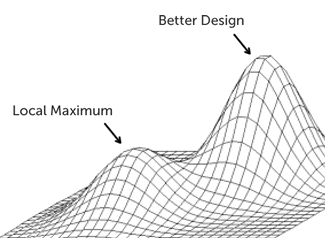
\includegraphics[width=0.65\textwidth]{img/intro/hill_climbing}
\caption{Hill-climbing algorithm local optimum}
\end{center}
\end{figure}
Modern algorithms have mechanisms that tackle this problem. An example of an algorithm that employ such mechanisms is simulated annealing. The simulated annealing is very similar to hill-climbing except that it occassionally accepts solutions that are worse than the current. Over time, the probability of accepting such solutions decreases. This allows for the avoidance of getting stuck in a local optimum.

The simulated annealing algorithm is modeled after the cooling process of a molten substance, and is one of many algorithms based on natural processes. Others include the genetic algorithm, ant colony optimization, and particle swarm optimization. For centuries humans have relied on nature to find the most appropriate solutions to problems. That's why in the past decades, computer scientists has turned to nature to develop novel algorithms.

\section{No Free Lunch Theorems}
Since there are already so many optimization algorithms, what's the point of making a new one? The No Free Lunch Theorems were introduced in 1997 by Wolpert and Macready to address the need for newer optimization algorithms. The first of their theorems states that for any pair of algorithms $a_1$ and $a_2$, iterated $m$ times, $$ \sum_{f} P(d_{m}^{y}|f,m,a_1)=\sum_{f} P(d_{m}^{y}|f,m,a_2),$$ where $d_m^y$ denotes the set of size $m$ of the cost values $y\in Y$ associated to the input values $x\in X,f:X\to Y$ is the function being optimized and $P(d_m^y|f,m,a)$ is the conditional probability of obtaining a given sequence of cost values from algorithm $a$ run $m$ times on function $f$. Essentially, this says that when all functions $f$ are equally likely to be used, the probability of observing an arbitrary sequence of cost values over the course of optimization is independent of the algorithm.
This theorem indicates that if an algorithm performs better than another algorithm on some class of problems, then it must perform worse on the remaining problems. Consequently, this implies that there is no general-purpose optimization algorithm that is universally superior than the rest. Hence, the development of newer optimization algorithms is still needed.

\section{Optimization: Genetic Algorithm}
The genetic algorithm \cite{holland_2010} is modeled after Darwin’s theory of evolution. An initial population is initialized in which each individual represents a solution to the problem. Through a series of selection, crossover, and mutation, successive populations are generated until an individual with a desired fitness is obtained. Fitness is defined as how well an individual can solve the given problem.

Selection pertains to the process in which individuals with the best fitness are selected and allowed to pass their genes (or properties. E.g. bits) to the next generation. The individuals with the highest fitness have a higher chance of being selected.

Crossover is when genes of the selected individuals are interchanged with each other. The results are called offspring and are added to the next generation.

Mutation refers to when genes of the offspring are subject to mutate or change (e.g. Binary value from 1 to 0). This further diversifies the sample space and consequently prevents the algorithm from converging early.

\section{Optimization: Particle Swarm Optimization}
The Particle Swarm Optimization \cite{eberhart_kennedy_1995} algorithm is modeled after the movement of a swarm as a whole (e.g. A flock
of birds collectively foraging for food). In this algorithm, an initial set of particles is first initialized with each
particle having a random initial velocity. These particles are then flung through hyperspace where each of their position
represents a solution to the problem at hand. Each of these solutions are evaluated regarding their fitness and a particle's
current most fit solution is stored as its 'pbest'. The current best solution attained by the entire set particles is also stored; this is called 'gbest'. For each time step of the algorithm, each particle is accelerated towards its 'pbest' and the 'gbest'. Eventually, these particles will converge around an optimal solution.

\section{Optimization: Artificial Immune Systems}
Artificial immune systems are a classification of rule based machine learning systems inspired by the vertebrate immune systems. This systems model the learning and memory for use in problem solving. These systems adapt to what they learn in the environment to become better at solving problems. Compared to GA these methods use less mutation per generation whenever the fitness becomes better.

\section{Optimization: Ant Colony Optimization}
Ants can find food faster by utilizing shorter paths found by the other ants in its colony. An ant would leave more pheromones when it has reached the food faster so other ants would be more inclined to use the path. This also applies to optimization by using memory and prioritizing directions with more incentives.

\section{Optimization: Marriage in Honey Bee Optimization}
The model simulates the evolution of honey-bees starting with a solitary colony (single queen without a family) to the emergence of an eusocial colony (one or more queens with a family).

\section{Optimization: Lion Pride Optimizer}
Previous works such as the Lion Pride Optimizer was inspired by this brutal competition of male lions whom also plays an important role for the persistence of the pride. In the work, the optimization chooses two of the best points in a ``pride'' and each ``female'' with a mating coefficient will create 4 offsprings only to choose one at last based on the best male in the pride. The optimization also uses safeguards to prevent stagnation in the pride by either replacing all members in the pride or resetting the search space.

\section{Optimization: Lion's Algorithm}
The lion's algorithm by Rajakumar \cite{rajakumar_2012} is another inspiration for the LOA. This algorithm is modeled after the territorial behavior of a lion pride, where the pride represents the solution space and a lion represents a solution. The pride is first initialized with one male and one female lion. Through mating, four cubs are generated as a result of single point crossover with dual possibilities. Four more cubs are generated from the mutation of these cubs, totalling eight cubs. These cubs are then grouped according to gender, and the weakest cubs are killed. A cub needs 2-4 years to reach maturity and so the territorial lions must defend the territory for the same number of years. During this time, nomadic lions may invade the pride. For each year, a nomadic lion is generated to test the strength of the pride. If the nomadic lion is found to be stronger than the territorial lions, the nomadic lion takes over the pride and kills the territorial lions' cubs. If the cubs survive and they mature, the best male and female lions take over the entire pride while the rest are killed.

\section{Applications}
Researchers have made good use of optimization problems such as scheduling problems, data clustering, image and video processing, tuning of neural networks, and pattern recognition.

\section{Application: Scheduling Problems}
Scheduling problems are problems where different difficulty on jobs would take different amount of time that will be processed by different nodes. The problem is to minimize the time that all the nodes would simultaneously get to be finished. Optimization helps find the best job to node assignment to minimize the mean time.

\section{Application: Data Clustering}
Data clustering or cluster analysis is the way to group a set of objects such that objects with the most similarity a group together in clusters. The objects may have one or more properties to identify and the groups may have smaller subgroups that one can also classify. Optimization helps identify the best clustering of an object based on its parameters.

\section{Application: Image and Video Processing}
Image and video processing is the process of adding metadata to an image or video based to what its visual content actually is. An image or video in a computer is represented as pixels or boxes of colors that is displayed on the screen of the viewer. These pixels individually cannot determine the actual content, which is significant to the viewer, of the image and video. Optimization algorithms help computers identify what pixels in an image or video actually represents to the viewer. Such algorithms help with edge detection, segmentation, representation and description of the parts of an image or video.

\section{Application: Tuning of neural networks}
Neural networks can be tuned by its parameters. These parameters talked about are parameters that are constant throughout the run of the network. This parameters may be tuned to get the best performance out of neural network which may also drive the network to learn faster, slower or not at all. Optimization helps to find the best parameters that will drive the system's performance.

\section{Application: Pattern Recognition}
Patterns can be also found in data. These patterns can help add to the metadata of that data. Pattern recognition finds those patterns that can be found off the data. Optimization helps identify patterns that best identify a given data.

\section{Inspiration for the algorithm}
Lions have displayed cooperation and antagonism especially in hunting. Lions are also socially inclined meaning that they also organize information that other lions have collected and use them for their benefit.
Male lions have radically different social behavior and appearance than the female lions and v.v.
The lions can also be classified if they're residents or nomads. Resident lions create groups called prides, establish their territories and flourish there while nomads take what they need in an area then finds another area to pillage not establishing territories.
A pride typically would include five females have cubs of both sexes and one or more adult male lions.
As young males would grow they would separate from their birth pride and establish their own prides.
Nomads, who doesn't establish territories, would move about sporadically (whenever they want) and either in pairs or singularly.
Lions usually hunt together in prides. Female lions would work together to surround and swiftly catch the prey. There could also be a hunter female lion who would go out of territory to hunt on their own while the other members of the pride would wait for the lioness to return. But still, coordinated group hunting would bring greater success in prey hunts.
Lions do go mate anytime around the year and females can have more than one reproductive cycle each year. A lioness can also mate with more than one lion when in heat.
Additionally, to mark their territory the pride would place urine all over the place to drive away others who would intrude.

\section{Idea for the algorithm}
The initially proposed algorithm started an initial population formed by a set of solutions randomly generated labelled as Lions.A percentage $\%N$ of the initial population of solutions are selected as `Nomad Lions' while the rest are the `Resident Lions'. While the nomad lions are individually grouped, the resident lions are then further divided into partitions called `Prides' where a percentage $\%S$ is percentage of the females in the group but in nomad lions, this percentage is reversed, where $\%S$ will be used to identify the males in the nomad lions.
Each lion will have a variable pertaining to the best obtained solution for every passing iteration that will be called best visited position and will be updated regularly for every iteration. In each pride, a few random females will be selected to go hunting. These females will encircle the prey and catch it. The males in the pride will roam the territory. The females may mate with one or more resident males then a young male is created. These males may establish their own prides and territory later or may become a nomad.
The nomad lions roams around the search space to find better (places) solutions. A nomad lion may invade and replace a resident male in a pride, driving out that resident male (replacement). Also, a female lion may also migrate to another pride or become a nomad herself. Weak lions, who have not found better prey (solutions) where there is no competition, will die or be killed (stagnation). The process will go on until the stopping condition is satisfied.

\section{Opposition Based Learning}
Opposition based learning is a novel idea of using opposite entities to arrive to better solutions or to arrive at the best solution faster. OBL is used to arrive to the best solution faster than the naive method. In Genetic Algorithm, OBL is also used to get better solutions by allowing multiple best solutions determined using the cost or revenue function to try predict better solutions influenced by the selected solutions' genes. A basic example of OBL is finding a solution $X$ in a one dimensional solution set. For the solution $\hat{X}$, we have an estimate $\hat{X}$ that approaches $X$ from the left. As we optimize to the solution $X$, the difference between the solution $X$ and the estimate $\hat{X}$ will get less and less as $\hat{X}$ gets near to the solution $X$. Suppose we get to $X$ at a certain time, which is the time from the start of the optimization to whenever the estimate $\hat{X}$ will be equal to the solution $ X $. If we use OBL and add another estimate $\hat{X}_2$ that would approach $X$ from the right then the time it takes for the optimization to arrive at solution $X$ would be the maximum between the time it takes for $\hat{X}$ or $\hat{X}_2$ to reach solution $X$.

\section{Proposed Algorithm: Initialization}
The first step of the algorithm is to randomly generate solutions called Lions with a population of N. In a Nvar dimensional search space optimization problem a Lion is represented as
$$Lion = [x_1, x_2,..., x_{Nvar}]$$
As most optimization algorithms, there will be a given cost function, where the fitness value of a solution can be gauged.
$$\text{fitness} = f(\text{Lion}) = f(x_1, x_2,..., x_{Nvar})$$
Along with generating the solutions, a percentage of $N$ will be selected as nomad lions and the rest would be divided into a number $P$ of prides. The solutions in the pride will have a specific gender which will identify their role in finding solutions. A percentage $S$ of the prides in the population are labeled as females (others are males) while in nomads will have the ratio reversed where $1-S$ will be the percentage of females in the nomads. The percentage $\%S$ is typically chosen between 75 to 90 percent.

\section{Proposed Algorithm: Hunting}
In a pride, females would look for a prey to provide food for the pride. The females would fill specific roles to execute certain strategies to encircle the prey and catch it. In general, lions would approximately follow a pattern in hunting. Stander divided lions into seven different stalking roles which would be grouped into by the Left Wings, Centers and Right Wings.
Left Wings and Right Wings both attack the prey from opposite directions in which the idea of Opposition Based Learning is utilized which also is proven to effectively solve optimization problems.
The group with members of the highest finesses (highest revenue, lowest cost) is considered as the Centers while the other two groups are considered as Left and Right Wings.
In the algorithm, the hunters are divided into three groups: Left, Right and Center. The group with highest cumulative finesses is considered to be the Center and the other groups would be Left and Right Wings.
\begin{figure}[h]
\begin{center}
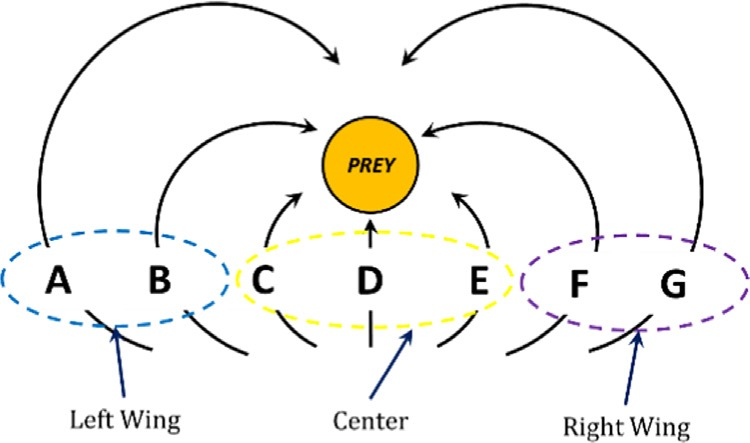
\includegraphics[width=0.65\textwidth]{img/pa/hunting_scheme}
\caption{Generalized lion hunting behavior}
\end{center}
\end{figure}
A dummy prey would move to a new position and escape as follows:
$$\text{PREY}' = \text{PREY} + \text{rand}(0,1) \times \text{PI} \times (\text{PREY} - \text{Hunter})$$
where PREY is the current position of the prey, PREY$'$ is the new position and PI is the percentage of improvement of the finesse of the hunter.
For the left and right wings, they approach the prey as follows:
\[ \text{Hunter}' =  \begin{cases} 
      \text{rand}((2 \times \text{PREY} - \text{Hunter}), \text{PREY}) & (2 \times \text{PREY} - \text{Hunter}) < \text{PREY} \\
      \text{rand}(\text{PREY}, (2 \times \text{PREY} - \text{Hunter})) & (2 \times \text{PREY} - \text{Hunter}) > \text{PREY}
   \end{cases}
\]
where Hunter is the current position of the hunter and Hunter' is the new position of the hunter.
As for the Center hunters, their new position is as follows:
\[ \text{Hunter}' =  \begin{cases} 
      \text{rand}(\text{Hunter}, \text{PREY}) & \text{Hunter} < \text{PREY} \\
      \text{rand}(\text{PREY}, \text{Hunter}) & \text{Hunter} > \text{PREY}
   \end{cases}
\]
In all of these equations, $\text{rand}(a,b)$ generates a random number between $a$ and $b$, where $a$ and $b$ are upper and lower bounds, respectively.
In the algorithm, this prey would be a dummy prey put at the start of the phase where PREY would be the midpoint between all the Hunter positions. Each of the hunters would be iterated to attack the dummy prey and the prey would escape to the direction opposite to the new position of the attacking Hunter from the Prey's current position.
\begin{figure}[h]
\begin{center}
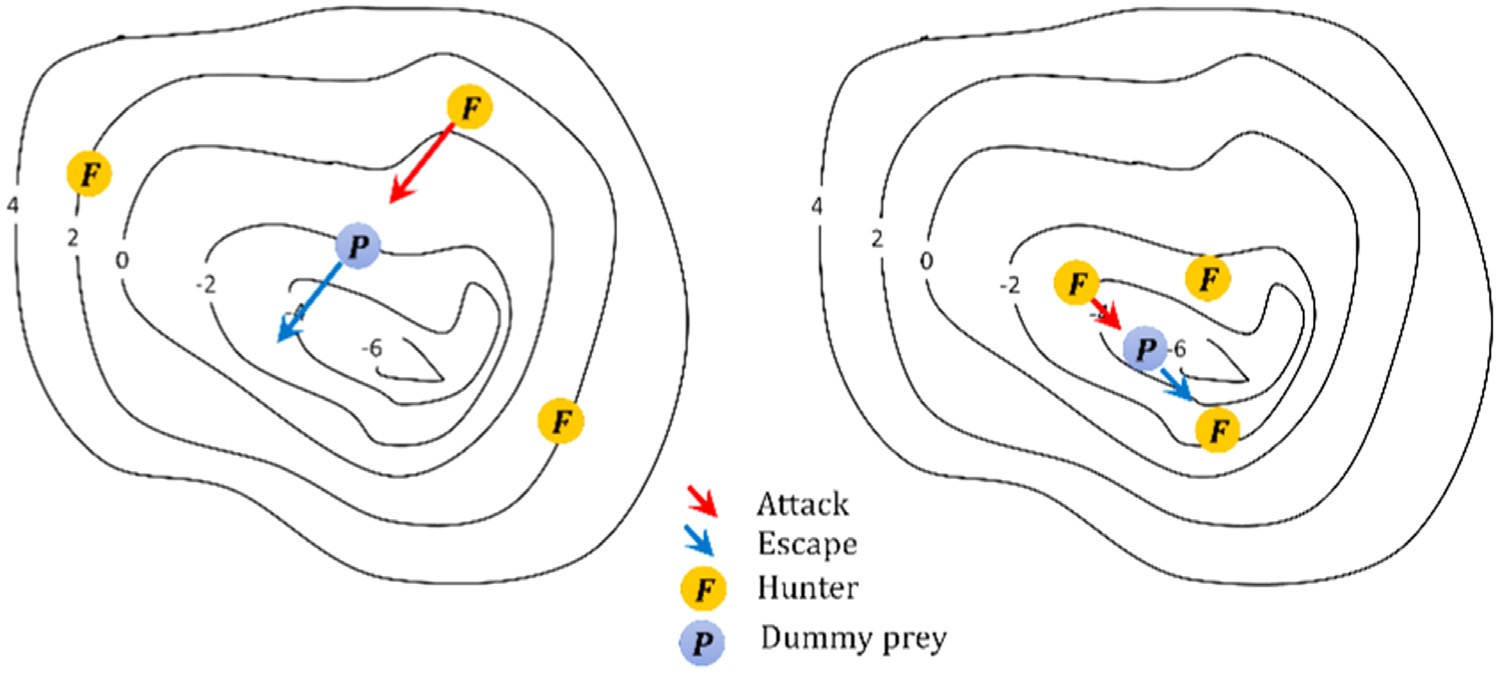
\includegraphics[width=0.65\textwidth]{img/pa/hunting_attack}
\caption{Attack and Escape Example}
\end{center}
\end{figure}
This mechanism allows the hunters to create a circle shaped neighborhood around the prey, approach it from different directions and catch it. This also allows better solutions to be found (escape local optima) because some hunters use opposite positions.
Therefore hunting in each pride can be stated in the following Pseudo-code:
\begin{figure}[h]
\begin{center}
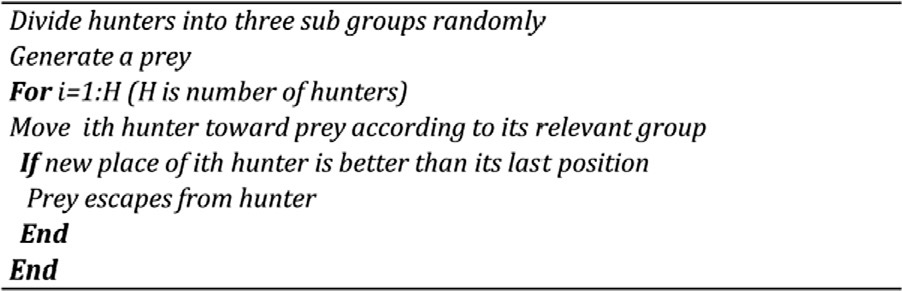
\includegraphics[width=0.65\textwidth]{img/pa/hunting_pseudo}
\end{center}
\end{figure}

\section{Proposed Algorithm: Moving towards safe place}

As mentioned earlier, some of the females go hunting, not all. So, remaining females go toward one of the areas of the territory. In the algorithm, the territories of each pride would consist of personal best solutions so far, which would assist the algorithm to save the best solutions obtained so far over the course of iteration.
Therefore the new position for a female lion is given as:
\begin{align*}
\text{Female Lion}' &= \text{Female Lion} + 2D \times rand(0,1){R1} + U(-1,1) \times \tan(\theta) \times D \times {R2} \\
&\text{  where } R1 \cdot R2 = 0, ||R2|| = 1
\end{align*}
where Female Lion and Female Lion' is the previous and next position of the female lion, respectively, and D is the distance between the female lion's position and the selected point chosen by tournament selection in the pride's territory.
{R1} is a vector which its start point is the previous location of the female lion and its direction is toward the selected position. {R2} is perpendicular to {R1}. $\theta$ is an angle that is selected by uniform distribution among $-\pi/6$ and $\pi/6$ and $U$ is a function selecting a random number with uniform distribution.


\section{Proposed Algorithm: Roaming}
\begin{comment}
Male lions in a pride would typically roam the pride's territory. To emulate this specific behavior of resident males, $\%R$
\end{comment}
--This section still requires further understanding--
